\documentclass{article}
\usepackage{amsfonts,amsmath,amssymb,amsthm}
\usepackage{ragged2e}
\usepackage{enumerate}
\usepackage{tikz}
\usepackage{pgfplots}
\usetikzlibrary{positioning}
\usetikzlibrary{hobby}
\usetikzlibrary{decorations.pathreplacing,calligraphy}
\usetikzlibrary{decorations.markings}
\usepackage[justification=centering]{caption}
\usepackage{bbm}
\usepackage{mathrsfs}
\usepackage{mathtools}
\usepackage{hyperref, xurl}
\usepackage{graphicx}
\usepackage{subcaption}
\usepackage{tocloft}
\usepackage{etoolbox}
\usepackage{needspace}

%Prevents footnotes from breaking across pages
\interfootnotelinepenalty=10000

%For the pgfplotset package to draw plots
\pgfplotsset{compat=1.18}

%Link colors
\hypersetup{
    colorlinks = true,
    linkcolor = black,
    citecolor = black,
    urlcolor = black
}


%custom colors 
\definecolor{custom_green}{rgb}{0.0, 0.5, 0.0}
\definecolor{custom_blue}{rgb}{0.2, 0.2, 0.6}
\definecolor{custom_blue2}{rgb}{0.16, 0.32, 0.75}
\definecolor{cardinal}{rgb}{0.77, 0.12, 0.23}

% new \oset macro:
\makeatletter
\newcommand{\oset}[3][0ex]{%
  \mathrel{\mathop{#3}\limits^{
    \vbox to#1{\kern-2\ex@
    \hbox{$\scriptstyle#2$}\vss}}}}
\makeatother

% Absolute value bars command. Write \abs{x}.
\DeclarePairedDelimiter\abs{\lvert}{\rvert}

%Real, complex, natural numbers and integers symbols
\newcommand{\R}{\mathbb{R}}
\newcommand{\Z}{\mathbb{Z}}
\newcommand{\C}{\mathbb{C}}
\newcommand{\N}{\mathbb{N}}

%Theorems, lemmas etc.
\newtheorem{theorem}{Theorem}[section]
\newtheorem{lemma}[theorem]{Lemma}
\newtheorem{proposition}[theorem]{Proposition}
\newtheorem{corollary}[theorem]{Corollary}
\theoremstyle{definition}
\newtheorem{definition}[theorem]{Definition}
\newtheorem{example}[theorem]{Example}
\theoremstyle{remark}
\newtheorem{remark}[theorem]{Remark}
\newtheorem*{claim}{Claim}

%Change default caption under figures/tables to be smaller
\captionsetup[figure]{font=small}

\begin{document}
    \tableofcontents
    \newpage

    This is a collection of statements I have proven myself and considered to be useful in some cases. I will often only present proof sketches instead of fully detailed proofs.

    \section{On manifolds with boundary}
    In this section we discuss how known theorems/lemmas fail for manifolds with non-emtpy boundary and how they can be generalized.
    
    \subsection{Regular values}
    It is known that for the regular value theorem, and more generally statements about transversality, to still hold for manifolds with boundary one needs to impose additional conditions on the boundary behaviour of a smooth function $f \colon M \to N$. Here is another lemma, that fits into the same category. We call $q \in N$ a \textbf{boundary value} of $f$ if $q \in f(\partial M)$.

    \begin{lemma}
        \label{lem:regular_sublevel_sets}
        Let $M$ be a manifold with boundary and $f \colon M \to \R$ a smooth function. Furthermore, let $a \in \R$ be a regular value of $f$, that is not a boundary value. Then $M_a := f^{-1}(-\infty,a]$ is a submanifold with boundary $\partial M_a = f^{-1}(a)$.
    \end{lemma}
    \begin{proof}[Proof sketch]
        For $p \in f^{-1}(a)$ we have $p \in \mathrm{int}(M)$ by assumption. Since $\mathrm{int}(M)$ is a boundaryless manifold the local submersion theorem holds, i.e. $f$ looks like the orthogonal projection $\R^n \to \R$ around $p$. Then the proof goes the same as in the boundaryless case.
    \end{proof}

    \begin{remark}
        To see that Lemma \ref{lem:regular_sublevel_sets} fails without the assumption that $a$ is not a boundary value consider $M := S^1 \times [0,1]$ and $f \colon M \to \R, (z,t) \mapsto t$. Then $f$ is everywhere regular but $f^{-1}(-\infty,0]$ does not satisfy the statements in Lemma \ref{lem:regular_sublevel_sets}. 
    \end{remark}
    \subsection{Morse Theory}

    
    For a smooth function $f \colon M \to \R$ and a regular value $a \in \R$ that is not a boundary value we define the \textbf{sublevel set} of $a$ to be
    \[
    M_a := f^{-1}(-\infty,a].
    \] 
    Lemma \ref{lem:regular_sublevel_sets} guarantees, that $M_a$ is a (sub-)manifold with boundary.

    \begin{lemma}
        \label{lem:topology_sublevel_sets_not_crossing_critical_point}
        Let $M$ be a compact manifold with boundary and $f \colon M \to \R$ a Morse function. Furthermore let $a,b \in \R$ be regular values of $f$, such that $[a,b]$ does not contain any critical values nor any boundary values. Then 
        \[
        M_a \cong M_b.
        \]
    \end{lemma}

    \begin{proof}
        Let $K := f^{-1}[a,b]$ and let $U := \{p \in \mathrm{int}(M) \mid p \text{ is a regular point of } f\}$. Then $U \subseteq M$ is open and $K \subseteq U$. Choose a cutoff function $\phi \colon M \to \R$ with
        \begin{itemize}
            \item $\phi|_{K} = 1$
            \item $\mathrm{supp}(\phi) \subseteq U$
            \item $0 \leq \phi \leq 1$
        \end{itemize}
        Now choose a pseudo gradient\footnotemark $X$ of $f$ and define the smooth vector field
        \[
            Y := \phi \frac{-1}{X \cdot f} X,
        \]


        \footnotetext{Here we agree to the convention that $X \cdot f < 0$ outisde of critical points.}

        \noindent which we define to be $0$ outside of $U$. Since $Y$ vanishes in a neighbourhood around $\partial M$ (or more generally since $Y$ is tangent to $\partial M$, see \cite{lee2011smooth} Theorem 9.34) we can consider the flow of $Y$: 
        \[
        \theta \colon M \times \R \to M.
        \]
        Since $M$ is compact (and $Y$ tangent to $\partial M$) each integral curve is defined for all time. Let $\theta_t := \theta( - ,t) \colon M \to M$. We claim that 
        \begin{align}
            \label{eq:flow1}
            \theta_{b-a}(M_b) \subseteq M_a, \\
            \label{eq:flow2}
            \theta_{a-b}(M_a) \subseteq M_b.
        \end{align}
        Let $p \in f^{-1}[a,b]$ and let $\gamma_p \colon \R \to M$ be the integral curve of $Y$ starting at $p$. Consider
        \[
        h \colon \R \to \R, \; t \mapsto f(\gamma_p(t)).
        \]
        Then for $t \in \R$ with $h(t) \in [a,b]$ we have $\phi(\gamma_p(t)) = 1$ and thus
        \[
        h^\prime(t) = \dot{\gamma_p}(t) \cdot f = Y_{\gamma_p(t)} \cdot f = -1.
        \]
        So $h$ is a smooth function with $c := h(0) = f(p) \in [a,b]$ and $h^\prime(t) = -1$ as long as $h(t) \in [a,b]$. We claim that $h(c-a) = a$. To see this let 
        \[
        s := \mathrm{sup}\{t \in [0,c-a] \mid h([0,t]) \subseteq [a,b]\}.
        \]
        Assume $s < c-a$. For continuity reasons we get that $h([0,s]) \subseteq [a,b]$ and thus $h^\prime(t) = -1$ for $t \in [0,s]$. Then $h(t) = c -t$ for $t \in [0,s]$. But then $h(s) \in (a,b]$ and $h$ is strictly decreasing around $t =s$ such that there exists $\epsilon >0$ with $h([0,s+\epsilon]) \subseteq [a,b]$, contradicting the definition of $s$. So $s = c-a$ and we get that $h(t) = c-t$ for $t \in [0,c-a]$. Thus $h(c-a) = a$.

        As $h^\prime(t) \leq 0$ for all $t \in \R$ we conclude
        \[
        f(\theta_{b-a}(p)) = h(b-a) \leq h(c-a) = a,
        \]
        thus $\theta_{b-a}(p) \in M_a$. For $p \in M_b \setminus f^{-1}[a,b] = \mathrm{int}{M_a}$ we also have 
        \[
        \theta_{b-a}(p) \in M_a
        \]
        as $f$ decreases along gradient flow lines of $Y$. This shows (\ref{eq:flow1}). We argue similiarly for (\ref{eq:flow2}). Let $p \in M_a$ and let $\gamma_p \colon \R \to M$ be the integral curve of $Y$ starting at $p$. Consider
        \[
        h \colon \R \to \R, \; t \mapsto f(\gamma_p(-t)).
        \]
        Then $h^\prime(t) = \phi(\gamma_p(-t)) \leq 1$. Assume that $h(b-a) = f(\theta_{a-b}(p)) > b$. Then by the mean value theorem there exists some $\xi \in [0,b-a]$ with 
        \[
        h^\prime(\xi) = \frac{h(b-a) - h(0)}{b-a} \geq \frac{h(b-a) - a}{b-a} > 1,
        \]
        which is a contradiction. So $f(\theta_{a-b}(p)) \leq b$, showing (\ref{eq:flow2}). Thus $\theta_{b-a}$ restricts to a diffeomorphism $M_b \oset[1pt]{\cong}{\longrightarrow} M_a$ with inverse $\theta_{a-b}$.
    \end{proof}

    \begin{counterexample}
        Example \ref{ex:boundary_values} also shows, that we need to impose conditions on the boundary values in Lemma \ref{lem:topology_sublevel_sets_not_crossing_critical_point}. To see that we also need that condition for Lemma \ref{lem:topology_sublevel_sets_not_crossing_critical_point_variation} we may similiarly define $f$ as the height function on the disjoint union of two cylinders which are slightly shifted in height. Similiar examples show, that Theorem \ref{thm:topology_when_crossing_critical_point} fails without the assumption on boundary values.
    \end{counterexample}

    \begin{remark}
        We can weaken the assumptions of Lemma \ref{lem:topology_sublevel_sets_not_crossing_critical_point}. First of all $f$ does not need to be a Morse function. We can then still construct a vector field $X$, such that $X \cdot f < 0$ outisde of critical points. Secondly, we may replace the assumption that $M$ is compact by instead requiring $f^{-1}[a,b]$ to be compact, which is for example the case if $f$ is proper. We then only have to modify the proof in the definition of $U$. Instead we define $U$ to be a \textit{compact} neighbourhood of $K := f^{-1}[a,b]$, i.e. $K \subseteq \mathrm{int} U$, which does not contain any critical points nor boundary points. For example we may define $U$ as a union of finitely many (here we need compactness of $f^{-1}[a,b]$) compact sets $K_i$ not containing neither critical points nor boundary points such that $\mathrm{int} K_i$ still cover $K$. 
    \end{remark}

    Similiarly we may proof the following, for which we can also weaken the assumptions as described in the remark above.

    \begin{lemma}
        \label{lem:topology_sublevel_sets_not_crossing_critical_point_variation}
        Let $M$ be a compact manifold with boundary and $f \colon M \to \R$ a Morse function. Furthermore let $a,b \in \R$ be regular values of $f$, such that $[a,b]$ does not contain any critical values nor any boundary values. Then 
        $M_a$ is a (not necessarily smooth) deformation retract of $M_b$.
    \end{lemma}
    \begin{proof}
        We consider the flow $\theta$ as in Lemma \ref{lem:topology_sublevel_sets_not_crossing_critical_point} and define a retraction
        \[
            r \colon M_b \to M_a, \; p \mapsto \begin{dcases}
            \theta(f(p) - a,p), & f(p) \geq a \\
            p, & f(p) \leq a
        \end{dcases}
        \]
        As we have shown above $\theta(f(p) - a,p) \in f^{-1}(a)$. It follows that $r$ is continous and well-defined. To see that $r$ is a deformation retract consider
        \[
        H \colon M_b \times [0,1] \to M_b, (p,t) \mapsto \begin{dcases}
            \theta(t(f(p) - a),p), & f(p) \geq a \\
            p, & f(p) \leq a
        \end{dcases}
        \]
        Then $H(-,0) = id_{M_b}$ and $H(-,1) = r$.
    \end{proof}

    We would now also like to generalize the result, that the topology of $M$ changes by attaching a $\lambda$-cell when crossing a critical point $c_0$ of index $\lambda$ to compact manifolds with boundary. This statement can now be shown using the two lemmas above by requiring $f^{-1}[a,b]$ to only contain the critical point $c_0$ and no boundary points. The proof now works exactly the same as for the boundaryless case, see \cite{milnor1963morse}. Let us state the theorem for manifolds with boundary:
    
    \begin{theorem}
        \label{thm:topology_when_crossing_critical_point}
        Let $M$ be a compact manifold with boundary and $f \colon M \to \R$ a Morse function. Let $c_0 \in M$ be a critical point of $f$ of index $\lambda$ and $c := f(c_0)$ as well as $\epsilon > 0$, such that $f^{-1}[c-\epsilon,c+\epsilon]$ contains no boundary points and no critical points besides $c$. Then for $\epsilon$ sufficiently small $M_{c+\epsilon}$ has the homotopy type of $M_{c-\epsilon}$ with a $\lambda$-cell attached. More precisely, there exists an attaching map 
        \[
            \phi \colon S^{\lambda - 1} = \partial D^\lambda \to \partial M_{c-\epsilon}
        \] and a homotopy equivalence 
        \[
        r \colon M_{c+\epsilon} \to M_{c-\epsilon} \cup_\phi D^\lambda
        \]
        with homotopy inverse 
        \[
        \iota \colon M_{c-\epsilon} \cup_\phi D^\lambda \to M_{c+\epsilon},
        \]
        such that $r \circ \iota = id_{M_{c-\epsilon} \cup_\phi D^\lambda}$.
    \end{theorem}
    \begin{proof}[Proof Sketch]
        Following \cite{milnor1963morse} we first construct $F \colon M \to \R$, such that 
        $$F^{-1}(-\infty,c+\epsilon] = f^{-1}(-\infty,c+\epsilon] = M_{c+\epsilon}.$$
        Furthermore $F^{-1}[c-\epsilon,c+\epsilon]$ does not contain any critical points or boundary points, such that $F^{-1}(-\infty,c-\epsilon]$ is a deformation retract of $F^{-1}(-\infty,c+\epsilon]$ by Lemma \ref{lem:topology_sublevel_sets_not_crossing_critical_point_variation}. We then show that $M_{c-\epsilon} \cup_\phi D^\lambda$ is a deformation retract of $F^{-1}(-\infty,c-\epsilon]$ (or more precisely the image of $M_{c-\epsilon} \cup_\phi D^\lambda$ under an embedding is a deformation retract). This then shows that $M_{c-\epsilon} \cup_\phi D^\lambda$ is a deformation retract of $M_{c+\epsilon}$.
    \end{proof}
    
    However this does not yield a cell decomposition of $M$ as we do not know how the topology changes when crossing boundary points. Instead we can use the fact that any compact manifold without boundary admits a cell-decomposition directly, to proof the case when $M$ has non-empty boundary.

    \begin{theorem}[Cell-decompositions of Manifolds]
        \label{thm:cell_decomp}
        Let $M$ be compact manifold with or without boundary. Then $M$ has the homotopy type of a CW-complex.
    \end{theorem}

    \begin{proof}
        The case when $M$ has no boundary is shown in \cite{milnor1963morse}. If $\partial M \neq \emptyset$ we can argue as follows: consider the double $D(M)$ of $M$. Then $D(M)$ is a compact manifold without boundary. Now we construct a Morse function on $D(M)$. Choose a Morse function $f \colon M \to \R$ with $f \leq 0$ and $f(p) = 0$ if and only if $p \in \partial M$, such that $f$ has no critical points on the boundary. Such Morse functions always exist, see \cite{BA}. We can then glue $f$ and $-f$ together to get a Morse function $F$ on $D(M)$, again see \cite{BA}. Then $M \cong F^{-1}(-\infty,0]$ and $0$ is a regular value of $F$, allowing us to refer back to the boundaryless case, which tells us that every sublevel set $M_a$ for a regular value $a \in \R$ has the homotopy type of a CW-complex.
    \end{proof}

    \begin{remark}
        We may also formulate Theorem \ref{thm:topology_when_crossing_critical_point} and \ref{thm:cell_decomp} for handle bodies instead of CW-complexes. The proof is essentially the same but instead of constructing a deformation retract $F^{-1}(-\infty,c-\epsilon] \to M_{c-\epsilon} \cup_\phi D^\lambda$ one constructs a homeomorphism $F^{-1}(-\infty,c-\epsilon] \to M_{c-\epsilon} \cup_\phi D^\lambda \times D^{n-\lambda}$.
    \end{remark}

    
\subsection{Integral curves and flows}

\begin{lemma}[Existence of Integral curves]
    \label{lem:existence_integral_curves}
    Let $M$ be a manifold with boundary, $X$ a smooth vector field on $M$ and $p \in M$. Then there exists a unique maximal integral curve $\gamma \colon I \to M$ starting at $p$, where one of the four following cases holds for $a \leq 0 \leq b$:
    \begin{enumerate}[(i)]
        \item $I = (a,b)$
        \item $I = [a,b)$ and $\gamma(a) \in \partial M$
        \item $I = (a,b]$ and $\gamma(b) \in \partial M$
        \item $I = [a,b]$ and $\gamma(a),\gamma(b) \in \partial M$
    \end{enumerate}
\end{lemma}

\begin{remark}
    \label{rem:vector_field_example}
    In general it does not hold that $a < b$ in Lemma \ref{lem:existence_integral_curves} as illustrated by the following example. Consider  the lower halfspace $M := \R^2_{y \leq 0}$ and the vector field $X := \frac{\partial}{\partial x} + 2x \frac{\partial}{\partial y}$. Then for $p = (0,0)$ the integral curve is only defined for $t = 0$, since on $\R^2$ it would be given by $\gamma(t) = (t,t^2)$ but $t^2 > 0$ for $t \neq 0$.
    \begin{figure}[ht]
        \centering
        \label{fig:vector_field1}
        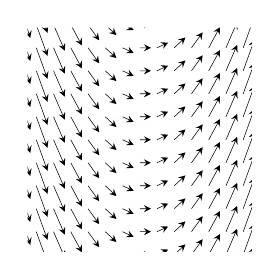
\begin{tikzpicture}[scale = 0.5,every plot/.append style={very thick}]
    \begin{axis}[
        clip = true,
        ticks = none,
        xmin = -1.5, xmax = 1.5,
        ymin = -1.5, ymax = 1.5,
        zmin = 0, zmax = 1,
        axis equal image,
        axis lines = middle,
        axis line style={draw=none},
        view = {0}{90},
    ]
        \addplot3[samples = 27,
            quiver = {
                u = {1},
                v = {2*x},
                scale arrows = 0.15,
            },
            -stealth,
            domain = -3:3,
            domain y = -4:4,
        ] {0};
    \end{axis}
    
\end{tikzpicture}
        \caption{The vector field $X$. The integral curves are parabolas.}
    \end{figure}
\end{remark}

\begin{proof}[Proof sketch of Lemma \ref{lem:existence_integral_curves}]
The proof is essentially the same as in the boundaryless case (see for example \cite{lee2011smooth}): We show that two integral curves $\gamma \colon I \to M$ and $\gamma^\prime \colon I^\prime \to M$ starting at $p$ agree on their common domain. This then allows us to define the maximal integral curve on some interval $I$ and every interval containing $0$ is of the form $(i) - (iv)$ \footnotemark. The only difference is that $I$ and $I^\prime$ may not be open intervalls. So we have to show that uniqueness still applies. We claim: Let $U \subseteq \R^n$ be open, $F \colon U \to \R^n$ a smooth vector field, $I$ an interval of the form $(i) - (iv)$ and $\gamma,\gamma^\prime \colon I \to U$ integral curves both starting at $p \in U$. Then $\gamma = \gamma^\prime$. If $0$ is an interior point of $I$ we can apply the usual uniqueness theorem for $\gamma,\gamma^\prime$ restricted to $\mathrm{int}(I)$. By continuity they must then also agree at the endpoint. So it remains to show uniqueness if $0$ is a boundary point of $I$ (say for example $I = [0,b)$). But by the existence theorem for integral curves we can find an integral curve $\eta \colon (-\epsilon,\epsilon) \to U$ starting at $p$ and define
\[
\beta \colon (-\epsilon,b) \to U, t \mapsto \begin{dcases*}
    \eta(t), t \leq 0 \\
    \gamma(t), t \geq 0
\end{dcases*}
\]
Since $\eta(0) = \gamma(0)$ and $\dot{\eta}(0) = F(p) = \dot{\gamma}(0)$ we get that $\beta$ is at least $C^1$. Similiarly we define
\[
\beta^\prime \colon (-\epsilon,b) \to U, t \mapsto \begin{dcases*}
    \eta(t), t \leq 0 \\
    \gamma^\prime(t), t \geq 0
\end{dcases*}
\]
By the uniqueness theorem we have
\[
\beta = \beta^\prime
\]
and our claim follows. The case $I = (a,0]$ goes analogous and for $I = [0,b]$ or $I = [a,0]$ it is either trivial (if $a = b = 0$) or we consider $I\setminus \{b\}$ resp. $I\setminus \{a\}$ and apply the above argument. Equality at $t = a, t = b$ respectively then again follows by continuity.

To see that $\gamma(t) \in \partial M$ for $t \in \{a,b\}$ a boundary point of $I$ we note that for $ p = \gamma(t) \in \mathrm{int}(M)$ we can define the integral curve starting at $p$ on some open interval $(-\epsilon,\epsilon)$ by the existence theorem for integral curves (Picard-Lindelöff). But then $t$ is not a boundary point of $I$ since $I$ is maximal.
    
\end{proof}

\footnotetext{If we put together integral curves defined on open intervals that agree on their common domain, it is clear that this results in a smooth curve, since around each $t$ this curve is given by one of the smooth curves which we put together. If we put together integral curves $\gamma_1,\gamma_2$ defined on something like $I_1 = (a,b]$ and $I_2 = [b,c)$ we have to be more careful around the boundary point $b$. But the same argument as we applied to $\beta$ in the proof of Lemma \ref{lem:existence_integral_curves} shows that putting $\gamma_1$ and $\gamma_2$ together results in a $C^1$-curve. We can then apply the usual uniqueness theorem to see that this curve is already given by a $C^\infty$-curve.}

On compact maniolds we can say more about the maximal Interval $I$:
\begin{lemma}[Existence of Integral curves on compact manifolds]
\label{lem:existence_integral_curves_compact_mnf}
    Let $M$ be a compact manifold with boundary, $X$ a smooth vector field on $M$ and $p \in M$. Then there exists a unique maximal integral curve $\gamma \colon I \to M$ starting at $p$, where one of the four following cases holds for $a \leq 0 \leq b$:
    \begin{enumerate}[(i)]
        \item $I = (-\infty,\infty)$
        \item $I = [a,\infty)$ and $\gamma(a) \in \partial M$
        \item $I = (-\infty,b]$ and $\gamma(b) \in \partial M$
        \item $I = [a,b]$ and $\gamma(a),\gamma(b) \in \partial M$
    \end{enumerate}
\end{lemma}
\begin{proof}
Let $\gamma \colon I \to M$ be the unique maximal integral curve guaranteed by Lemma \ref{lem:existence_integral_curves}. We will show that any open boundary point of $I$ must be $\pm \infty$. For simplicity let us only consider $I = [a,b)$. The other cases are completely analogous. By compactness we can find a sequence $0 < t_n \nearrow b$ such that $\gamma(t_n)$ coverges to a point $q \in M$.

\noindent \textbf{Case 1: $q \in \mathrm{int}(M)$.} By Picard-Lindelöff we can find an open neighbourhood $U \subseteq M$ around $q$ and $\epsilon > 0$, such that for every point $x \in U$ the intgeral curve starting at $x$ is defined for $t \in (-\epsilon,\epsilon)$. For some fixed $m$ sufficiently large we have $q_0 := \gamma(t_m) \in U$. Assume that $b - t_m < \frac{\epsilon}{2}$. But then we can extend $\gamma$ to $[a,b + \frac{\epsilon}{2})$ as follows. Consider
\[
\gamma^\prime \colon [a-t_m,b-t_m) \to M, \; t \mapsto \gamma(t + t_m).
\]
Then $\gamma^\prime$ is a integral curve starting at $q_0$. Let $\alpha \colon (-\epsilon,\epsilon) \to M$ be another integral curve starting at $q_0$. Then $\alpha$ and $\gamma^\prime$ agree on their common domain by the arguments in Lemma $\ref{lem:existence_integral_curves}$ and thus we can put them together to define an integral curve 
\[
\beta \colon J \to M
\]
for $J := [a-t_m,b-t_m) \cup (-\epsilon,\epsilon) \supseteq [a-t_m,\epsilon)$. But then we can define
\[
\gamma^{\prime\prime} \colon [a,\epsilon + t_m) \to M, \; t \mapsto \beta(t-t_m),
\]
which is an integral curve starting at $\gamma(0) = p$. However
\[
b + \frac{\epsilon}{2} < t_m + \epsilon
\]
and so $[a,b + \frac{\epsilon}{2}) \subseteq [a,\epsilon + t_m)$, contradicting maximality of $\gamma$.

\noindent \textbf{Case 2: $q \in \partial M$.} We argue similiarly as above. In a local chart around $q$ we can again apply Picard-Lindelöff (smoothness of $X$ guarantees by definition the existence of a smooth extension of $X$ to an open neighbourhood in $\R^n$). We then again take $q_0 := \gamma(t_m)$ sufficiently close to $q$, choose an integral curve $\alpha$ starting at $q$, which we can use to define an integral curve $\alpha^\prime$ starting at $q_0$ defined on some open interval $(-\epsilon,\epsilon) $ by translation in time as above. Also we define $\gamma^\prime$ as above. The same argument as above then shows that we can extend $\gamma^\prime$ (in the local chart) to an integral curve $\beta$ on $J := [a-t_m,b-t_m) \cup (-\epsilon,\epsilon) \supseteq [a-t_m,b-t_m]$. In particular we have $\beta([a-t_m,b-t_m]) \subseteq M$. Translating in time again yields an integral curve $\gamma^{\prime\prime} \colon [a,b] \to M$ contradicting maximality.
\end{proof}


\begin{remark}[A note on flows for manifolds with boundary]
    In general the concept of a flow is not well behaved if $M$ has boundary. Consider for example the vector field in Remark \ref{rem:vector_field_example}. Then the integral curve for $p = (0,0)$ is only defined for $t=0$ but for every other point it is defined on a half-open interval. In \cite{lee2011smooth} the author shows, that if $X$ is tangent to $\partial M$ we still get a well-behaved flow, i.e. it is defined on some open subset $\mathcal{O} \subseteq M \times \R$. I think that if we instead assume, that $X$ is transversal to $\partial M$, we still get a "good" flow domain in the sense that we can define the flow on some subset $\mathcal{D} \subseteq M \times \R$, which is a codimension $0$ submanifold with boundary and $I_p := \{ t \in \R \mid (p,t) \in \mathcal{D}\}$ is an interval for each $p \in M$.
\end{remark}

The statement in the above remark should follow from the following lemma, which allows us to define submanifold charts for $\mathcal{D}$.

\begin{lemma}
    Let $M$ be a manifold with boundary and $X$ a vector field of $M$, which is inward pointing along $\partial M$. Let 
    \[
    M_{\partial} := \{p \in M \mid \mathrm{im}\gamma_p \cap \partial M \neq \emptyset\}
    \]
    be all points in $M$ whose trajectory contains boundary points (this is at most one for each $p \in M$). For $p \in M_\partial$ the integral curve $\gamma_p$ starting at $p$ is defined on some interval $[-\tau(p),a)$ for some $\tau(p) \geq 0$ and $a > -\tau(p)$. Then the following statements hold true
    \begin{enumerate}[(i)]
        \item $M_\partial$ is an open subset of $M$
        \item $\tau \colon M_\partial \to \R_{\geq 0}, \, p \mapsto \tau(p)$ is smooth
    \end{enumerate}
\end{lemma}
\begin{proof}[Proof sketch]
    The idea is to consider the maximal flow
    \[
    \theta \colon \mathcal{D} \to M, \; (p,t) \mapsto \gamma_p(t)
    \]
    on some open subset $\mathcal{D} \subseteq \partial M \times [0,\infty)$ and show that this is an embedding. Then 
    \[
    M_\partial = \mathrm{im} \theta
    \]
    is open and 
    \[
    \tau = \pi \circ \theta^{-1} \colon M_\partial \to [0,\infty)
    \]
    for $\pi \colon \partial M \times [0,\infty) \to [0,\infty)$ is the canonical projection map.
\end{proof}
    
    \section{Miscellaneous}

    \subsection{Smoothness on arbitrary subsets}

Let $M,N$ be manifolds and $A \subseteq M$ an arbitrary subset. In \cite{lee2011smooth} the author defines what it means for a map
\[
f \colon A \to N
\]
to be smooth, namely
\begin{center}
    \textit{We call $f$ smooth if around each $x \in A$ there exists a smooth extension $\oset[-1pt]{\sim}{f} \colon U \to N$ of $f$ to some open neighbourhood $U \subseteq M$ of $x$ (see \cite[p. 45]{lee2011smooth}).}
\end{center}
However this definition has a fatal flaw: if $A$ happens to be a submanifold of $M$, a map $f \colon A \to N$ might be smooth in the usual sense (i.e. as a map between smooth manifolds) but not smooth in the sense of Lee`s definition. Consider for example
\begin{gather*}
    M := \R, N:= [0,1], A := [0,1], \\
    f \colon A \to N, \, t \mapsto t.   
\end{gather*}
Then clearly $f$ is smooth as a map between smooth manifolds, but around $0,1 \in A$ it does not admit a smooth extension onto an open neighbourhood $U \subseteq M$, since the image of such an extension would fail to be contained within $N$. We can however correct this flaw by defining:

\begin{definition}[Extension-smooth]
    \label{def:extension_smooth}
    Let $M^n,N^m$ be manifolds with or without boundary, $A \subseteq M$ an arbitrary subset and $f \colon A \to N$ a map. We call $f$ \textit{extension-smooth} if around each $x \in A$ there exist charts
    \begin{gather*}
        h \colon U \to M \text{ around } x\\
        k \colon V \to N \text{ around } f(x),
    \end{gather*}
    such that
    \[
    g:= k^{-1} \circ f \circ h|_{h^{-1}(A)}
    \]
    admits a smooth extension around $h^{-1}(x)$ in the sense that there exist open subsets $U_0 \subseteq \R^n$ and $V_0 \subseteq \R^m$ with $h^{-1}(x) \in U_0$ and $k^{-1}(f(x)) \in V_0$ and a smooth map 
    \[
    \oset[-1pt]{\sim}{g} \colon U_0 \to V_0
    \]
    with $g|_{U_0 \cap h^{-1}(A)} = \oset[-1pt]{\sim}{g}|_{U_0 \cap h^{-1}(A)}$.
\end{definition}

We now claim the following.

\begin{lemma}
    If $\partial N = \emptyset$ then Lee`s definition and Definition \ref{def:extension_smooth} are equivalent. In general Lee`s definition is stronger.
\end{lemma}

\begin{lemma}
    If $A$ is a submanifold of $M$, then $f \colon A \to N$ is smooth as a map of smooth manifolds if and only if it is extension-smooth.
\end{lemma}

In particular the extension Lemma in \cite{lee2011smooth} (Lemma 2.26.) still holds and the proof of the Whitney approximation theorems in chapter 6 work the same (here the extension Lemma is used). But with our new definition Problem 6-7 in \cite{lee2011smooth} now is an actual counterexample. (with Lee`s definition $F$ would not be smooth on the closed subset $A$ but only smooth as a map between manifolds).

Another way to properly define smoothness of $f \colon A \to N$ would be to change the codomain in Lee`s definition to be the double of $N$. This should be equivalent to Definition \ref{def:extension_smooth}.




% Add an unnumbered entry for the bibliography in the table of contents
\cleardoublepage
\addcontentsline{toc}{section}{References}

% Include all entries from BibTeX file
\nocite{*}

\bibliographystyle{alpha}
\bibliography{ref}
\end{document}